\documentclass{article}
% ---------- Core ----------
\usepackage{stackengine}
\usepackage{tikz}
\usetikzlibrary{fit}
\usepackage{multirow}
\usepackage{multicol}
\usepackage[margin=1in]{geometry}
% ---------- Text formatting ----------
% Gives some extra formatting options, e.g. underlining/strikeout
\usepackage{ulem}
\usepackage{setspace}
\onehalfspacing
\usepackage{array}

% Paragraph formatting
\usepackage[parfill]{parskip}
\setlength{\parskip}{5pt} % plus 1 minus 1}
\setlength{\parindent}{30pt}

\usepackage{titlesec}


% ---------- Math & symbols ----------
% Basic math symbols
\usepackage{pifont}
\usepackage{amssymb}
\usepackage{amsmath}
\newcommand{\defeq}{\mathrel{:=}}
%%% Gives shortcuts for glossing (optional)
% \usepackage{leipzig}

% ---------- Tables ----------
\usepackage{caption}   % For table captions
\usepackage{booktabs}  % Helps format tables

% ---------- Citations ----------
\usepackage{natbib}

% ---------- Fonts ----------
\usepackage{libertine}
% A font that actually contains many IPA symbols.

% Note: if using system fonts, compile with XeLaTeX

% ---------- Highlighting ----------
% Highlights text with \hl{text}
\usepackage{color, soul}

% ---------- Trees ----------
\usepackage[linguistics]{forest}
% Formatting for nicer trees
\forestset{
  nice nodes/.style={
    for tree={
      inner sep=0pt,
      fit=band,
    },
  },
  default preamble=nice nodes,
}

% ---------- Examples ----------
%% For numbered and glossed examples %%
\usepackage{gb4e}

%%%%%%%%%%%%
%% End of PREAMBLE
%%%%%%%%%%%%
\title{Logical Transductions for Tonal Patterns Triggered by Vowel Deletion}
\author{Han Li}
\date{}
\vspace{-3em}
\begin{document}
\maketitle
\section{Introduction}
Vowel hiatus is avoided in many languages through processes such as vowel
deletion or modification. In tonal languages, where vowels typically serve 
as tone-bearing units (TBUs), hiatus resolution often triggers changes in 
the association between tones and vowels. These include tone deletion, 
contour formation, and tone coalescence. Such patterns that linear phonology
has been struggled to capture have been extensively studied in autosegmental
phonology. From a autosegmental perspective, the tonal processes can be 
generalized by modifying the association relations between tones and vowels, 
which shows simpler generaiztions than changing the tonal or vocalic features 
themselves. This also demonstrates the distinct natures of tonal and segmental 
phonology.
In the previous computational phonology work, little work has been done to 
model tonal processes over autosegmental representations. This paper proposes 
that most of tonal processes can be computationally modeled by two logical
transduction: reassociation and deassociation. We show that these two 
operations can capture the three typologically common outcomes of vowel 
deletion, as well as less common patterns such as vowel deletion blocking. We 
further show how these processes can be learned using a structured hypothesis 
space, drawing connections to recent work on computational learning in 
phonology.


\section{Typology}
We argue that three typologically common outcomes of vowel deletion 
can be derived from two basic operations on association relations: 
\textit{deassociation} and \textit{reassociation}. Specifically:
\begin{enumerate}
    \item Tone deletion arises from deassociation without subsequent reassociation.
    \item Contour formation arises from reassociation of a tone to an already-associated TBU.
    \item Tone coalescence arises from reassociation together with constraints on tonal sequences.
\end{enumerate}

We further show that this system also applies to less common 
patterns. In particular, it captures cases of tone coalescence 
in Moba and Yoruba, as well as vowel deletion blocking 
in Ezinaihite Mbaise, where association relations constrain the 
applicability of the deletion process.

We formalize these processes as logical transductions and show how 
they operate over autosegmental representations with tone, vowel, 
and association relations. We then illustrate the analysis with 
case studies from typologically diverse languages. Finally, we 
outline how such processes can be learned using a structured 
hypothesis space, drawing connections to recent work on 
computational learning in phonology.


\begin{table*}[ht]
\centering
\begin{tabular}{l|ll}
\toprule
Process & Condition & Language \\
\midrule
\multirow{3}{*}{Tone Deletion}
    & Tone quality 
    & \\
    & Association faithfulness 
    & \\
    & Morphosyntax 
    & \\
\midrule
\multirow{2}{*}{Tone Retention}
    & Contour Formation
    & Ewe \\
    & Tone Coalescence
    & Moba, Yoruba \\
\bottomrule
\end{tabular}
\caption{Typology of tonal processes triggered by vowel deletion}
\end{table*}

\section{Logical Transduction}
\citet{yolyan2025logical} provides a general framework for modeling 
phonological maps over strings. The input and output strings are represented 
as relational structures, and the transduction is defined by a set of logical 
formulas that specify how the output structure is derived from the input 
structure. We follow \citeauthor{yolyan2025logical}'s formalization and apply
to AR using the common patterns.
\subsection{Tone Elision}
In languages that the vowel associated with the deleting vowels will also get 
deleted, this can be solved by a simple deassociation operation. The 
unassociated tone will stay unassociated without any further operation, which
will not be realized in the surface form. 

An example can be drawn from Engenni (Niger-Congo, Nigeria). When two 
vowels are adjacent, the first vowel always get deleted along with 
its associated tone. 

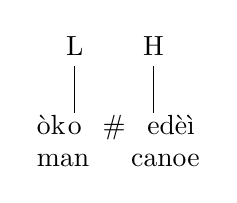
\begin{tikzpicture}
		\node (s1)[anchor=base] at (-.3, 0) {òk} ; 
        \node (s1)[anchor=base] at (0, 0) {o} ; 
		\node (gl1)[anchor=base] at (-.15, -.4) {man} ; 
		\node (wb)[anchor=base] at (0.5, 0) {\#} ; 
		\node (s2)[anchor=base] at (1, 0) {e} ; 
		\node (ss)[anchor=base] at (1.3, 0) {dèì} ; 
		\node (gl1)[anchor=base] at (1.15, -.4) {canoe} ; 
        \node[anchor=base] (t1) at (0,1) {L} ; 
        \node[anchor=base] (t2) at (1,1) {H} ;
	\draw (s1) -- (t1) ;
	\draw (s2) -- (t2) ;
\end{tikzpicture}
\hfill
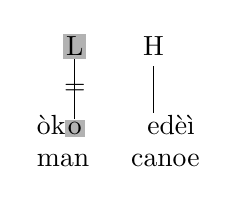
\begin{tikzpicture}
% grey highlight FIRST (so it stays behind)
% \fill[gray!20] (-0.15,-0.2) rectangle (0.3,1.5);
\node (s1a)[anchor=base] at (-.3, 0) {òk} ; 
\node (s1)[anchor=base, fill=black!30, inner sep=1pt] at (0, 0) {o};
\node (gl1)[anchor=base] at (-.15, -.4) {man} ; 
% \node (wb)[anchor=base] at (0.5, 0) {\#} ; 
\node (s2)[anchor=base] at (1, 0) {e} ; 
\node (ss)[anchor=base] at (1.3, 0) {dèì} ; 
\node (gl2)[anchor=base] at (1.15, -.4) {canoe} ; 

\node[anchor=base, fill=black!30, inner sep=1pt](t1) at (0,1) {L} ; 
\node[anchor=base] (t2) at (1,1) {H} ;

\draw (s1) -- (t1) node[midway] {$=$} ;
\draw (s2) -- (t2) ;
\end{tikzpicture}
\hfill
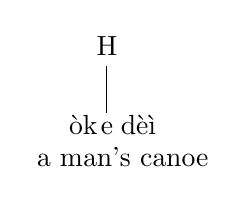
\begin{tikzpicture}
		\node (s1)[anchor=base] at (0, 0) {òk} ; 
        % \node (s1)[anchor=base] at (0, 0) {o} ; 
		\node (gl1)[anchor=base] at (.5, -.4) {a man's canoe} ; 
		\node (s2)[anchor=base] at (.3, 0) {e} ; 
		\node (ss)[anchor=base] at (.7, 0) {dèì} ; 
		% \node (gl1)[anchor=base] at (1.15, -.4) {canoe} ; 
        % \node[anchor=base] (t1) at (0,1) {L} ; 
        \node[anchor=base] (t2) at (.3,1) {H} ;
	% \draw (s1)[dotted] -- (t1) ;
	\draw (s2) -- (t2) ;
\end{tikzpicture}
\begin{figure}[ht]
\centering
\begin{tabular}{>{\centering\arraybackslash}m{3cm}
                >{\centering\arraybackslash}m{3cm}
                >{\centering\arraybackslash}m{3cm}
                >{\centering\arraybackslash}m{3cm}}

% Graph 1
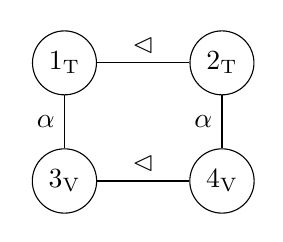
\begin{tikzpicture}
\node[circle, draw] (t1) at (0,1.5) {1\textsubscript{T}};
\node[circle, draw] (t2) at (2,1.5) {2\textsubscript{T}};
\node[circle, draw] (v1) at (0,0) {3\textsubscript{V}};
\node[circle, draw] (v2) at (2,0) {4\textsubscript{V}};
\draw (t1) -- node[midway, left] {$\alpha$} (v1);
\draw (t1) -- node[midway, above] {$\lhd$} (t2);
\draw (t2) -- node[midway, left] {$\alpha$} (v2);
\draw (v1) -- node[midway, above] {$\lhd$} (v2);
\end{tikzpicture}

&

% Structure 1
\[
\begin{aligned}
\mathcal{D} &= \{1,2,3,4\} \\
T &= \{1,2\} \\
V &= \{3,4\} \\
\lhd_T &= \{\langle 1,2\rangle\} \\
\lhd_V &= \{\langle 3,4\rangle\} \\
\alpha &= \{(1,3),(2,4)\}
\end{aligned}
\]

&

% Graph 2
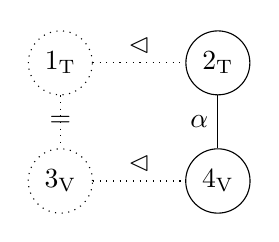
\begin{tikzpicture}
\node[circle, draw, dotted] (t1) at (0,1.5) {1\textsubscript{T}};
\node[circle, draw] (t2) at (2,1.5) {2\textsubscript{T}};
\node[circle, draw, dotted] (v1) at (0,0) {3\textsubscript{V}};
\node[circle, draw] (v2) at (2,0) {4\textsubscript{V}};
\draw[dotted] (t1) -- node[midway] {$=$} (v1);
\draw[dotted] (t1) -- node[midway, above] {$\lhd$} (t2);
\draw (t2) -- node[midway, left] {$\alpha$} (v2);
\draw[dotted] (v1) -- node[midway, above] {$\lhd$} (v2);
\end{tikzpicture}

&

% Structure 2
\[
\begin{aligned}
\mathcal{D} &= \{2,4\} \\
T &= \{2\} \\
V &= \{4\} \\
\alpha &= \{(2,4)\}
\end{aligned}
\]

\end{tabular}
\end{figure}





A transduction for tone deletion can be defined as follows:

\begin{align*}
	% \phi_{\textsf{license}}(x) \defeq& \text{True}\\
	% \textit{C} \defeq& 2 \\
	H'(x) := & H(x)\\
	L'(x) := & L(x)\\
	V'(x) := & V(x) \land \neg \textsf{delete\_V} (x)\\
	\lhd_T'(x,y) := & \lhd_T(x,y) \\
	\lhd_V'(x,y) := & \lhd_V(x,y) \\
	\alpha'(x,y) := & \alpha(x,y) \land \neg \textsf{deassoc }(x,y) \text{ where}\\
	\textsf{deassoc}(T,V) := & \alpha(T,V) \land \textsf{delete\_V}(V) \\
\end{align*}

It should be mention that the deletion condition is language specific. For
the example, Engenni deletes the proceeding vowel in the hiatus and in other 
language the following. These two conditions can be captured by the following formulas respectively:

Engenni: $\textsf{delete\_V}(V) := \exists V' s.t \lhd(V',V) $\\
L2: $\textsf{delete\_V}(V) := \exists V' s.t \lhd(V,V') $\\
L3: $\textsf{delete\_V}(V) := \exists V s.t a(V) \land \lhd(V',V) \lor \lhd(V,V')$\\


As can be seen from the tranduction, everything stays the same except the 
association relation. The deassociation and reassociation conditions are 
what determine the output association relation. For the contour formation

\begin{align*}
	\textsf{deassoc}(T,V) := & \alpha (T,V) \land  \exists V' \text{st} \lhd(V',V) \land \neg \alpha (T,V') \\
	\textsf{reassoc}(T,V) := & \neg \alpha (T,V) \land  \exists V' \text{st} \lhd(V,V') \land \alpha (T,V') \\
\end{align*}

\subsection{Contour Formation}
Vowel deletion is a common remedy for vowel hiatus, which often further
results in tonal instability. As a result, the tone associated with the deleted 
vowel may disassociate from the deleted vowel and reassociate to the surviving 
vowel, resulting in a contour formation. The contour usuallay follows the linear
order of two tones. Based on Hao, all languages in the survey but not reversed 
order. The logical transduction for contour formation is as follows:


Contour tone formation in Etsako 

\begin{tikzpicture}
        \node (s1) at (0, 0) {V_1} ; 
		\node (wb) at (0.5, 0) {\#} ; 
		\node (s2) at (1, 0) {V_2} ; 
        \node[anchor=base] (t1) at (0,1) {T_1} ; 
        \node[anchor=base] (t2) at (1,1) {T_2} ;

	%association lines
	% \draw [dotted, thick] (s1) -- (t2) ;
	\draw (s1) -- (t1) ;
	\draw (s2) -- (t2) ;
\end{tikzpicture}
\hfill
\begin{tikzpicture}
        \node (s1) at (0, 0) {V_1} ; 
		\node (s2) at (1, 0) {V_2} ; 
        \node[anchor=base] (t1) at (0,1) {T_1} ; 
        \node[anchor=base] (t2) at (1,1) {T_2} ;

	%association lines
	\draw [dotted, thick] (s1) -- (t2) ;
	\draw (s1) -- (t1) ;
	\draw (s2) -- (t2) node[midway] {$=$} ;
\end{tikzpicture}
\hfill
\begin{tikzpicture}
        \node (s1) at (0, 0) {V_1} ; 
		\node (s2) at (1, 0) {V_2} ; 
        \node[anchor=base] (t1) at (0,1) {T_1} ; 
        \node[anchor=base] (t2) at (1,1) {T_2} ;

	%association lines
	\draw [thick] (s1) -- (t2) ;
	\draw (s1) -- (t1) ;
	% \draw (s2) -- (t2) node[midway] {$=$} ;
\end{tikzpicture}



\begin{tikzpicture}
        \node (s1) at (0, 0) {V_1} ; 
		\node (wb) at (0.5, 0) {\#} ; 
		\node (s2) at (1, 0) {V_2} ; 
        \node[anchor=base] (t1) at (0,1) {T_1} ; 
        \node[anchor=base] (t2) at (1,1) {T_2} ;

	%association lines
	% \draw [dotted, thick] (s1) -- (t2) ;
	\draw (s1) -- (t1) ;
	\draw (s2) -- (t2) ;
\end{tikzpicture}
\hfill
\begin{tikzpicture}
        \node (s1) at (0, 0) {V_1} ; 
		\node (s2) at (1, 0) {V_2} ; 
        \node[anchor=base] (t1) at (0,1) {T_1} ; 
        \node[anchor=base] (t2) at (1,1) {T_2} ;

	%association lines
	\draw [dotted, thick] (s2) -- (t1) ;
	\draw (s1) -- (t1) node[midway] {$=$} ;
	\draw (s2) -- (t2) ;
\end{tikzpicture}
\hfill
\begin{tikzpicture}
        \node (s1) at (0, 0) {V_1} ; 
		\node (s2) at (1, 0) {V_2} ; 
        \node[anchor=base] (t1) at (0,1) {T_1} ; 
        \node[anchor=base] (t2) at (1,1) {T_2} ;

	%association lines
	\draw [thick] (s2) -- (t2) ;
	\draw (s2) -- (t1) ;
\end{tikzpicture}

\begin{align*}
	% \phi_{\textsf{license}}(x) \defeq& \text{True}\\
	% \textit{C} \defeq& 2 \\
	H'(x) := & H(x)\\
	L'(x) := & L(x)\\
	V'(x) := & V(x)\\
	\lhd_T'(x,y) := & \lhd_T(x,y) \\
	\lhd_V'(x,y) := & \lhd_V(x,y) \\
	\alpha'(T,V) := & (\alpha(T,V) \land \neg \textsf{deassoc}(T,V)) \lor \textsf{reassoc}(T,V) \\		
\end{align*}
As can be seen from the tranduction, everything stays the same except the 
association relation. The deassociation and reassociation conditions are 
what determine the output association relation.

For the contour formation
\begin{align*}
	\textsf{deassoc}(T,V) := & \alpha (T,V) \land  \exists V' \text{st} \lhd(V',V) \land \neg \alpha (T,V') \\
	\textsf{reassoc}(T,V) := & \neg \alpha (T,V) \land  \exists V' \text{st} \lhd(V,V') \land \alpha (T,V') \\
\end{align*}

\bibliography{ref}
\bibliographystyle{apalike}
\end{document}
